% Use only LaTeX2e, calling the article.cls class and 12-point type.

\documentclass[12pt]{article}

% Users of the {thebibliography} environment or BibTeX should use the
% scicite.sty package, downloadable from *Science* at
% www.sciencemag.org/about/authors/prep/TeX_help/ .
% This package should properly format in-text
% reference calls and reference-list numbers.

\usepackage{scicite}

% Use times if you have the font installed; otherwise, comment out the
% following line.

\usepackage{times}

\usepackage{graphicx}

% The preamble here sets up a lot of new/revised commands and
% environments.  It's annoying, but please do *not* try to strip these
% out into a separate .sty file (which could lead to the loss of some
% information when we convert the file to other formats).  Instead, keep
% them in the preamble of your main LaTeX source file.


% The following parameters seem to provide a reasonable page setup.

\topmargin -1.0cm
\oddsidemargin 0.0cm
\textwidth 16cm 
\textheight 23cm
\footskip 1.0cm

%The next command sets up an environment for the abstract to your paper.

\newenvironment{sciabstract}{%
\begin{quote} \bf}
{\end{quote}}

% If your reference list includes text notes as well as references,
% include the following line; otherwise, comment it out.

%\renewcommand\refname{References and Notes}

% The following lines set up an environment for the last note in the
% reference list, which commonly includes acknowledgments of funding,
% help, etc.  It's intended for users of BibTeX or the {thebibliography}
% environment.  Users who are hand-coding their references at the end
% using a list environment such as {enumerate} can simply add another
% item at the end, and it will be numbered automatically.

\newcounter{lastnote}
\newenvironment{scilastnote}{%
  \setcounter{lastnote}{\value{enumiv}}%
  \addtocounter{lastnote}{+1}%
  \begin{list}%
  {\arabic{lastnote}.}
  {\setlength{\leftmargin}{.22in}}
  {\setlength{\labelsep}{.5em}}
}
{\end{list}}

\title{Lab Work 1} 

\author
{André Pedrosa [85098], Filipe Pires [85122], João Alegria [85048]\\
\\
Algorithmic Information Theory\\
\normalsize{Department of Electronics, Telecommunications and Informatics}\\
\normalsize{University of Aveiro}\\
} 

\date{\today{}}

%%%%%%%%%%%%%%%%% END OF PREAMBLE %%%%%%%%%%%%%%%%

\begin{document} 

% Double-space the manuscript.

\baselineskip18pt

% Make the title.

\maketitle 

% Place your abstract within the special {sciabstract} environment.

%\begin{sciabstract}
  
%\end{sciabstract}

% In setting up this template for *Science* papers, we've used both
% the \section* command and the \paragraph* command for topical
% divisions.  Which you use will of course depend on the type of paper
% you're writing.  Review Articles tend to have displayed headings, for
% which \section* is more appropriate; Research Articles, when they have
% formal topical divisions at all, tend to signal them with bold text
% that runs into the paragraph, for which \paragraph* is the right
% choice.  Either way, use the asterisk (*) modifier, as shown, to
% suppress numbering.

\section*{Introduction}

This report aims to describe the work developed for the first assignment
of the discipline of 'Algorithmic Information Theory', explaining all the 
steps and decisions taken by us, and presenting the results we considered 
most relevant.

The programs implemented in C++ have the purpose of collecting statistical
information about texts using Markov (finite-context) models, and of 
automatically producing texts that follows the models built.

Along with the description of the solution, we also discuss the effects
of the variation of the programs' parameters and attempt to compare 
different types of texts by the amount of information they hold on average.
\newpage

\section*{1. Information Model}

Our first goal was to be able to predict the next outcome of a text source.
To do this, we needed to take in consideration the dependencies between 
the characters of a text.
The use of Markov models for the extraction of the statistical properties of a
text was due to its value as an approach to represent these data dependencies.

The specific type of model that most interests us is called discrete time
Markov chain or finite-context model.
This model assigns a probability estimate to the symbols of the alphabet, 
according to a conditioning context computed over a finite and fixed number
of past outcomes. 
More about this is explained in the description of this work assignment 
\cite{trab1}, containing the mathematical equations that served as the basis 
for our implementation.

\subsection*{1.1. Collecting Data}

We decided to organize the program by several files, each with a different
purpose, for good readability and to allow future modifications without the 
need of much refactoring - so we adopted a modular architecture strategy.

The file \texttt{fcm.cpp} serves as the base code for the command to be executed in order to 
generate a finite-context model, given one or several information source(s).
By executing this command, the program is started and begins to
call a set of functions that return an instance of our 
implementation of the Markov's model trained from the information source(s), 
and calculate the text entropy, as estimated by this instance.
The \texttt{fcm} command has the following format:

\begin{quote}
\begin{verbatim}
$ ./fcm.cpp [-h] k alpha trainFile [trainFile ...]
\end{verbatim}
\end{quote}

Here, \texttt{-h} is the option that presents the manual for the command usage.
Argument \texttt{k} is the value given for the size of the context.
This context corresponds to a string with \texttt{k} characters, it is based on
the several contexts produced and on the single characters that follow each one
of them that the model is able to calculate the text's entropy.
\texttt{alpha} stands for the value of the 'smoothing' parameter for estimating
the probabilities of events. 
These events correspond to the occurrences of a character after a given context.
And \texttt{trainFile} is, as the name indicates, the name of the file(s) that
contain the text to be processed by the model.

First, the command executed is pre-processed and its arguments are collected
and validated by the function {\it parseArguments()\/}, implemented in 
\texttt{argsParsing.cpp} and defined in \texttt{argsParsing.h}.
The use of a header file is to establish an interface for the possibility of
creating different implementations of the parsing functions.
This is also visible in the implementation of the Model class in files 
\texttt{model.cpp} and \texttt{model.h}.

Once the arguments are validated, the program attempts to open the file(s) for reading
through function {\it checkAccess()\/} and, in case of success, reads and parses
its content.
The program supports any file format as long as its content is plaintext.

\newpage 
Below we present the actual implementation in C++ of the function responsible 
for parsing the information source file.

Variable \texttt{abc} contains the alphabet of the input file, updated everytime
a new character is found.
The function {\it parseFile()\/} creates a copy of this alphabet and a new
alphabet that will contain the new found characters (if any).
It then iterates over the file's content letter by letter, inserts each on both
alphabets (if not already in them), updates the number of occurrences of each 
letter after the corresponding context and updates total number of contexts in 
each iteration.
Once the end of file (EOF) is reached, the function calls 
{\it calcProbabilitiesAndEntropy()\/}.

\begingroup
\addtolength\leftmargini{-0.4in}
\addtolength\baselineskip{-0.05in}
\begin{quote}
\begin{verbatim}
  void Model::parseFile(list<fstream*> &input) {
    [...]
    for (auto reader : input) {
        while (reader->get(letter)) {
            abc.insert(letter);
            if (context.length() >= ctxLen) {
                statsTable[context].nextCharStats[letter].count++;
                statsTable[context].stats.count++;
                totalContextsCount++;
                context = context.substr(1);
            }
            context += letter;
        }
    }
    calcProbabilitiesAndEntropy();
  }
\end{verbatim}
\end{quote}
\endgroup

This solutions makes our model prepared to accept more than one information
source (i.e. several input files).
Although this was not a requirement, we knew this would make the program more
robust and scalable.

\newpage

\subsection*{1.2. Training the Model and Returning Text Entropy}

Finally, as the file is parsed and the alphabet is built, \texttt{fcm} then 
builds the information table containing the statistics of the input text and
calculates the estimated value for the entropy through the function
{\it calcProbabilitiesAndEntropy()\/}. To build the information table we
followed a dictionary approach where we have a first level dictionary where
the key is the context string and the value is a structure 
(ConstextStatistics) that contains a structure (Statistics) with statistics
(number of occurrences and probability) of that context and a dictionary.
This second layer dictionary has as key a letter of the alphabet and as value
the statistics structure mentioned before, but this time the data is relative
to appearances of a letter after a given context.

As all context's and letter's number of occurrences are calculated on the
method {\it parseFile()}, on the {\it calcProbabilitiesAndEntropy()} method we
calculate their probabilities. Context's probability is given by its
number of occurrences divided by the sum of appearances of all contexts, in
other words, the total number of contexts in all training data. Letter's
conditional probability is obtained dividing the number of occurrences of a
letter after a given context by the number of occurrences of that context.

To calculate these probabilities we iterate over the two layer dictionary.
On the first layer of the dictionary we calculate probabilities related to
contexts (\(P(c)\)) and while iterating over the second layer we calculate
the context entropy (\(H_c\)). For a given context not all letters of the
alphabet appear after it, to fix this we did a copy of the alphabet
and removed the ones that appeared and set the their count to 0 and
calculated the conditional probability.

The conditional probability mentioned is affected by a smoothing parameter
which allows letters that did not appear after a context to have a
higher than 0 probability.

Calculating all this prevent us from having to iterate over the entire table
again to calculate the model entropy or the conditional probabilities for
letters after a context.

The mathematical equations required for the calculation of the entropy are available in the document that describes the assignment. 
% The actual work was to implement these formulas and apply them.

The function {\it calcProbabilitiesAndEntropy()\/} is presented next for further
analysis.

\begingroup
\addtolength\leftmargini{-0.4in}
\addtolength\baselineskip{-0.05in}
\begin{quote}
\begin{verbatim}
  void Model::calcProbabilitiesAndEntropy() {
    [...]
    for (auto &it : statsTable) {
        contextStats = &it.second;
        contextCount = contextStats->stats.count;
        contextStats->stats.probability = 
          (double)contextCount / totalContextsCount;
        set<char> abcCopy(abc);
        for (auto &it2 : contextStats->nextCharStats) {
            letter = it2.first;
            stats = &it2.second;
            charCount = stats->count;
            conditionalProb = 
              (charCount + alpha) / (contextCount + alpha * abc.size());
            stats->probability = conditionalProb;
            Hc += conditionalProb * log2(conditionalProb);
            abcCopy.erase(letter);
        }
        for (char l : abcCopy) {
            conditionalProb = alpha / (contextCount + (alpha * abc.size()));
            contextStats->nextCharStats[l] = {0, conditionalProb};
            if (conditionalProb > 0) {
                Hc += conditionalProb * log2(conditionalProb);
            }
        }
        Hc = -Hc; 
        entropy += contextStats->stats.probability * Hc;
        Hc = 0.0;
    }
  }
\end{verbatim}
\end{quote}
\endgroup
\newpage

\section*{2. Text Generator}

The second part of the assignment was to developed a program for automatic
text generation that follows the statistical model learned beforehand using 
a training text.
To do this, we use \texttt{model.cpp} as a starting point and developed 
\texttt{generator.cpp}. 
This program, similarly to \texttt{fcm}, works as a command when executed.
\texttt{generator} similarly to fcm starts by passing the information source(s) to the model, that
internally will construct the model by calculating the probabilities of each character of the alphabet
knowing that a context appened, with the same dataflow as the fcm program when processing the file. 
After the model and the calculations are complete, the program begins to generate text,
starting with the text passed by the user and generating as much characters as the user intended.

The \texttt{generator} command has the following format: 

\begin{quote}
\begin{verbatim}
$ ./generator.cpp [-h] k alpha beginSequence numChars \\
outputFile trainFile [trainFile ...]
\end{verbatim}
\end{quote}

Once again we have the \texttt{-h} option that presents the manual for the 
command usage.
Arguments \texttt{k} and \texttt{alpha} are the same as the ones on the 
command \texttt{fcm}.
The \texttt{beginSequence} argument asks the user to give a word or character
sequence for the program to start off from; this is a need instrinsic to the
way the solution works and must be the same length as the context lenght.
The \texttt{numChars} argument tells the program how many characters are to be outputed.
The \texttt{outputFile} is where the generated text will be written to.
Finally the \texttt{trainFile} is, as the name suggests, the name of the file(s) to be
processed by the model and used as training.

\section*{3. Results}

In this chapter we discuss the results achieved from the final version of 
both tasks solutions. 
During development, we used randomly generated texts to test our code.
However, for the analysis described here, we used two text files
containing {\it The Bible\/} in plaintext, one written in English 
(\texttt{bible\_en\_v1.txt}) and the other in Portuguese 
(\texttt{bible\_pt.txt}).
The reason we chose the same text source translated in different languages
was to evaluate the entropy of each language and compare them in terms of 
average quantity of information per character of the alphabet.
These files suffered a minor pre-processing in order to make their formats 
as similar as possible.

\subsection*{3.1. Parameter Variation}

We defined a few assumptions after considering the problem of determining
the entropy of an information model and aimed to test them out once the 
program was completed.
In this section we explain these hipothesis and analyse their truthfulness
with the aid of a graphic plotting the evolution of the text entropy with
parameters k and alpha as variables.
It is important to state that our assumptions are based on the interpretation
of the mathematical formulas around the model implemented and that they 
are supposed to apply to texts of any size.

Taking a closer look at the formula for the overal entropy of the model 
(equation 1), we can gather that as the context probability 
decreases so does the value of the entropy.
But what exactly affects the probability of a context? 
Assuming we start from an equal probability of occurring any of the existing
contexts, the more contexts there are, the less probability there is of 
occurring a specific one.
Also, for a given text source, the longer the context is (substring of fixed 
size from the text source), the more possible combinations of letters there 
are and, consequently, the more unique contexts appear on the given text.
Taking this in consideration, we are able to establish that increasing the 
context size results in an increase of the total number of different contexts
and, consequently, in a decrease of the probability of occurring each context
and finally leading to a decrease in the final value for the model's entropy
(see equation 2).

\begin{equation}
  H = \sum\limits_{c} P(c) Hc
\end{equation}
\begin{equation}
  >size(c) \Rightarrow <P(c) \Rightarrow <H
\end{equation}

Our second hypothesis regarded the 'smoothing' parameter alpha.
The idea behind this parameter is to tackle the issue of constructing the
model and assigning zero probability to unseen events.
By adding alpha, the character probabilities is uniformized and they 
never actually reach zero.
As we studied the effects of the variable on the formula of conditional 
probabilities (see equation 3), we came to the conclusion that the larger
its value, the bigger will be the model's entropy.

\begin{equation}
  P(e|c) \approx \frac{N(e|c) + \alpha}{\sum\limits_{s\in\Sigma}N(s|c) + \alpha|\Sigma|}
\end{equation}

This was harder to reach as, at first sight, the effect of alpha is only 
relevant in a binary way, i.e. it affects the result if it is bigger than 
zero (the same way, no matter its value), it does not if not.
However, by analysing the situation more carefully, we understood that,
assuming that alpha is bigger than zero, the larger its value, the smaller
is the bottom parcel of equation 3 and, consequently the larger the 
conditional probability is.
From that point on, one can understand that the larger the alpha, the larger
will be the entropy.\\

We developed a script in \texttt{Matlab} that runs \texttt{fcm.cpp} a
defined number of times for the same source of information varying the 
two studied parameters in several combinations.
This script collects the entropy values for each combination and then plots
them in a line graph.
Our next step was to run the script for the file \texttt{......}, varying
k between ....... and ....... , and alpha between ...... and ......... .
Figure \ref{graph} shows the resulting plot.

\begin{figure}[h!]
  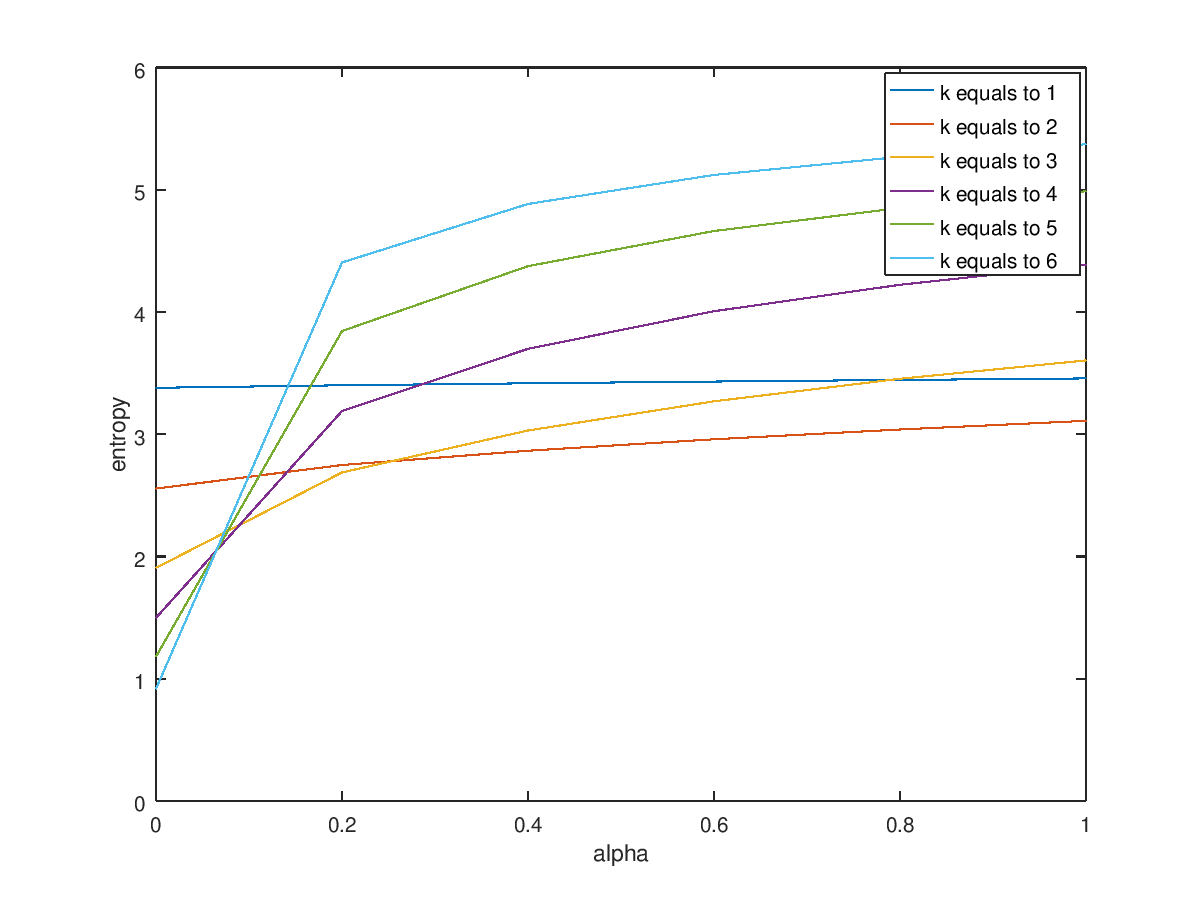
\includegraphics[width=\linewidth]{graph.png}
  \caption{............}
  \label{graph}
\end{figure}

grafico confirma, mas, para ks baixos, a segunda condicao nao se confirma
pq, como o texto é tao grande, 

.............

\subsection*{3.2. Text Comparison}

Lorem ipsum ...

\subsection*{3.3. Generator's Response to Parameter Variations}

Lorem ipsum ...

\section*{Conclusions}

Lorem ipsum ...

\begin{thebibliography}{9}
  \bibliographystyle{Science}

  \bibitem{trab1}
    Armando,
    \textit{AIT: Lab Work no.1},
    University of Aveiro,
    2019/20.
  
\end{thebibliography}


% In this file, we present some tips and sample mark-up to assure your
% \LaTeX\ file of the smoothest possible journey from review manuscript
% to published {\it Science\/} paper.  We focus here particularly on
% issues related to style files, citation, and math, tables, and
% figures, as those tend to be the biggest sticking points.  Please use
% the source file for this document, \texttt{scifile.tex}, as a template
% for your manuscript, cutting and pasting your content into the file at
% the appropriate places.

% {\it Science\/}'s publication workflow relies on Microsoft Word.  To
% translate \LaTeX\ files into Word, we use an intermediate MS-DOS
% routine \cite{tth} that converts the \TeX\ source into HTML\@.  The
% routine is generally robust, but it works best if the source document
% is clean \LaTeX\ without a significant freight of local macros or
% \texttt{.sty} files.  Use of the source file \texttt{scifile.tex} as a
% template, and calling {\it only\/} the \texttt{.sty} and \texttt{.bst}
% files specifically mentioned here, will generate a manuscript that
% should be eminently reviewable, and yet will allow your paper to
% proceed quickly into our production flow upon acceptance \cite{use2e}.


% \section*{Formatting Citations}

% Citations can be handled in one of three ways.  The most
% straightforward (albeit labor-intensive) would be to hardwire your
% citations into your \LaTeX\ source, as you would if you were using an
% ordinary word processor.  Thus, your code might look something like
% this:


% \begin{quote}
% \begin{verbatim}
% However, this record of the solar nebula may have been
% partly erased by the complex history of the meteorite
% parent bodies, which includes collision-induced shock,
% thermal metamorphism, and aqueous alteration
% ({\it 1, 2, 5--7\/}).
% \end{verbatim}
% \end{quote}


% \noindent Compiled, the last two lines of the code above, of course, would give notecalls in {\it Science\/} style:

% \begin{quote}
% \ldots thermal metamorphism, and aqueous alteration ({\it 1, 2, 5--7\/}).
% \end{quote}

% Under the same logic, the author could set up his or her reference list as a simple enumeration,

% \begin{quote}
% \begin{verbatim}
% {\bf References and Notes}

% \begin{enumerate}
% \item G. Gamow, {\it The Constitution of Atomic Nuclei
% and Radioactivity\/} (Oxford Univ. Press, New York, 1931).
% \item W. Heisenberg and W. Pauli, {\it Zeitschr.\ f.\ 
% Physik\/} {\bf 56}, 1 (1929).
% \end{enumerate}
% \end{verbatim}
% \end{quote}

% \noindent yielding

% \begin{quote}
% {\bf References and Notes}

% \begin{enumerate}
% \item G. Gamow, {\it The Constitution of Atomic Nuclei and
% Radioactivity\/} (Oxford Univ. Press, New York, 1931).
% \item W. Heisenberg and W. Pauli, {\it Zeitschr.\ f.\ Physik} {\bf 56},
% 1 (1929).
% \end{enumerate}
% \end{quote}

% That's not a solution that's likely to appeal to everyone, however ---
% especially not to users of B{\small{IB}}\TeX\ \cite{inclme}.  If you
% are a B{\small{IB}}\TeX\ user, we suggest that you use the
% \texttt{Science.bst} bibliography style file and the
% \texttt{scicite.sty} package, both of which we are downloadable from our author help site
% (http://www.sciencemag.org/about/authors/prep/TeX\_help/).  You can also
% generate your reference lists by using the list environment
% \texttt{\{thebibliography\}} at the end of your source document; here
% again, you may find the \texttt{scicite.sty} file useful.

% Whether you use B{\small{IB}}\TeX\ or \texttt{\{thebibliography\}}, be
% very careful about how you set up your in-text reference calls and
% notecalls.  In particular, observe the following requirements:

% \begin{enumerate}
% \item Please follow the style for references outlined at our author
%   help site and embodied in recent issues of {\it Science}.  Each
%   citation number should refer to a single reference; please do not
%   concatenate several references under a single number.
% \item Please cite your references and notes in text {\it only\/} using
%   the standard \LaTeX\ \verb+\cite+ command, not another command
%   driven by outside macros.
% \item Please separate multiple citations within a single \verb+\cite+
%   command using commas only; there should be {\it no space\/}
%   between reference keynames.  That is, if you are citing two
%   papers whose bibliography keys are \texttt{keyname1} and
%   \texttt{keyname2}, the in-text cite should read
%   \verb+\cite{keyname1,keyname2}+, {\it not\/}
%   \verb+\cite{keyname1, keyname2}+.
% \end{enumerate}

% \noindent Failure to follow these guidelines could lead
% to the omission of the references in an accepted paper when the source
% file is translated to Word via HTML.

% \section*{Handling Math, Tables, and Figures}

% Following are a few things to keep in mind in coding equations,
% tables, and figures for submission to {\it Science}.

% \paragraph*{In-line math.}  The utility that we use for converting
% from \LaTeX\ to HTML handles in-line math relatively well.  It is best
% to avoid using built-up fractions in in-line equations, and going for
% the more boring ``slash'' presentation whenever possible --- that is,
% for \verb+$a/b$+ (which comes out as $a/b$) rather than
% \verb+$\frac{a}{b}$+ (which compiles as $\frac{a}{b}$).  Likewise,
% HTML isn't tooled to handle certain overaccented special characters
% in-line; for $\hat{\alpha}$ (coded \verb+$\hat{\alpha}$+), for
% example, the HTML translation code will return [\^{}$(\alpha)$].
% Don't drive yourself crazy --- but if it's possible to avoid such
% constructs, please do so.  Please do not code arrays or matrices as
% in-line math; display them instead.  And please keep your coding as
% \TeX-y as possible --- avoid using specialized math macro packages
% like \texttt{amstex.sty}.

% \paragraph*{Displayed math.} Our HTML converter sets up \TeX\
% displayed equations using nested HTML tables.  That works well for an
% HTML presentation, but Word chokes when it comes across a nested
% table in an HTML file.  We surmount that problem by simply cutting the
% displayed equations out of the HTML before it's imported into Word,
% and then replacing them in the Word document using either images or
% equations generated by a Word equation editor.  Strictly speaking,
% this procedure doesn't bear on how you should prepare your manuscript
% --- although, for reasons best consigned to a note \cite{nattex}, we'd
% prefer that you use native \TeX\ commands within displayed-math
% environments, rather than \LaTeX\ sub-environments.

% \paragraph*{Tables.}  The HTML converter that we use seems to handle
% reasonably well simple tables generated using the \LaTeX\
% \texttt{\{tabular\}} environment.  For very complicated tables, you
% may want to consider generating them in a word processing program and
% including them as a separate file.

% \paragraph*{Figures.}  Figure callouts within the text should not be
% in the form of \LaTeX\ references, but should simply be typed in ---
% that is, \verb+(Fig. 1)+ rather than \verb+\ref{fig1}+.  For the
% figures themselves, treatment can differ depending on whether the
% manuscript is an initial submission or a final revision for acceptance
% and publication.  For an initial submission and review copy, you can
% use the \LaTeX\ \verb+{figure}+ environment and the
% \verb+\includegraphics+ command to include your PostScript figures at
% the end of the compiled PostScript file.  For the final revision,
% however, the \verb+{figure}+ environment should {\it not\/} be used;
% instead, the figure captions themselves should be typed in as regular
% text at the end of the source file (an example is included here), and
% the figures should be uploaded separately according to the Art
% Department's instructions.


% \section*{What to Send In}

% What you should send to {\it Science\/} will depend on the stage your manuscript is in:

% \begin{itemize}
% \item {\bf Important:} If you're sending in the initial submission of
%   your manuscript (that is, the copy for evaluation and peer review),
%   please send in {\it only\/} a PostScript or PDF version of the
%   compiled file (including figures).  Please do not send in the \TeX\ 
%   source, \texttt{.sty}, \texttt{.bbl}, or other associated files with
%   your initial submission.  (For more information, please see the
%   instructions at our Web submission site,
%   http://www.submit2science.org/ .)
% \item When the time comes for you to send in your revised final
%   manuscript (i.e., after peer review), we require that you include
%   all source files and generated files in your upload.  Thus, if the
%   name of your main source document is \texttt{ltxfile.tex}, you
%   need to include:
% \begin{itemize}
% \item \texttt{ltxfile.tex}.
% \item \texttt{ltxfile.aux}, the auxilliary file generated by the
%   compilation.
% \item A PostScript file (compiled using \texttt{dvips} or some other
%   driver) of the \texttt{.dvi} file generated from
%   \texttt{ltxfile.tex}, or a PDF file distilled from that
%   PostScript.  You do not need to include the actual \texttt{.dvi}
%   file in your upload.
% \item From B{\small{IB}}\TeX\ users, your bibliography (\texttt{.bib})
%   file, {\it and\/} the generated file \texttt{ltxfile.bbl} created
%   when you run B{\small{IB}}\TeX.
% \item Any additional \texttt{.sty} and \texttt{.bst} files called by
%   the source code (though, for reasons noted earlier, we {\it
%     strongly\/} discourage the use of such files beyond those
%   mentioned in this document).
% \end{itemize}
% \end{itemize}

% Your references go at the end of the main text, and before the
% figures.  For this document we've used BibTeX, the .bib file
% scibib.bib, and the .bst file Science.bst.  The package scicite.sty
% was included to format the reference numbers according to *Science*
% style.

% \bibliography{scibib}

% Following is a new environment, {scilastnote}, that's defined in the
% preamble and that allows authors to add a reference at the end of the
% list that's not signaled in the text; such references are used in
% *Science* for acknowledgments of funding, help, etc.

% \begin{scilastnote}
% \item We've included in the template file \texttt{scifile.tex} a new
% environment, \texttt{\{scilastnote\}}, that generates a numbered final
% citation without a corresponding signal in the text.  This environment
% can be used to generate a final numbered reference containing
% acknowledgments, sources of funding, and the like, per {\it Science\/}
% style.
% \end{scilastnote}

% For your review copy (i.e., the file you initially send in for
% evaluation), you can use the {figure} environment and the
% \includegraphics command to stream your figures into the text, placing
% all figures at the end.  For the final, revised manuscript for
% acceptance and production, however, PostScript or other graphics
% should not be streamed into your compliled file.  Instead, set
% captions as simple paragraphs (with a \noindent tag), setting them
% off from the rest of the text with a \clearpage as shown  below, and
% submit figures as separate files according to the Art Department's
% instructions.

\clearpage

\end{document}




















